This chapter lists the requirements for the effects presented in the analysis. 

%\begin{figure}[htbp]
%	\centering
%\begin{picture}(0,0)%
%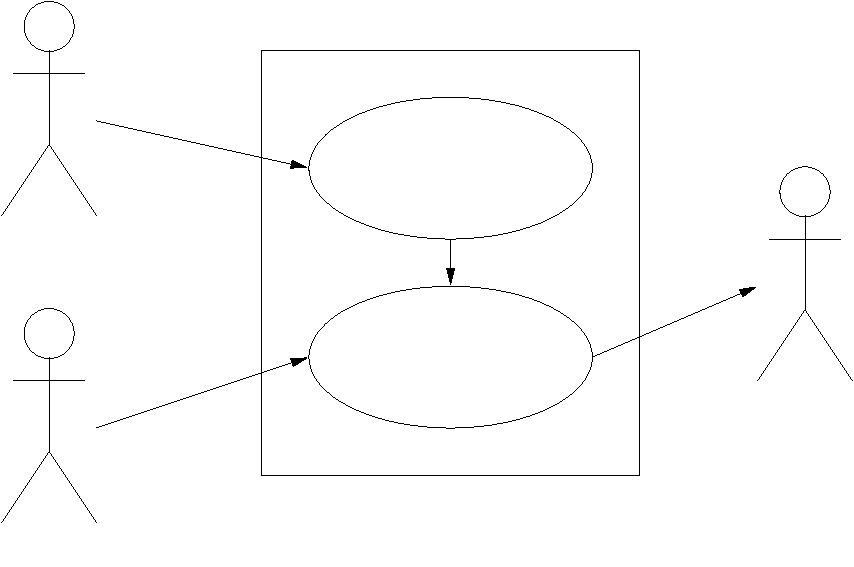
\includegraphics{Use_case.pdf}%
%\end{picture}%
%\setlength{\unitlength}{4144sp}%
%%
%\begingroup\makeatletter\ifx\SetFigFont\undefined%
%\gdef\SetFigFont#1#2#3#4#5{%
%  \reset@font\fontsize{#1}{#2pt}%
%  \fontfamily{#3}\fontseries{#4}\fontshape{#5}%
%  \selectfont}%
%\fi\endgroup%
%\begin{picture}(6507,4318)(1426,-4900)
%\put(1531,-2491){User}%
%\put(4546,-3346){Effect}%
%\put(4276,-1906){Effect select}%
%\put(7111,-3751){Amplifier}%
%\put(1441,-4831){Guitar}%
%\end{picture}%
%	\caption{A graphically overview of wanted functionality in form of an use case digram.}
%	\label{fig:use_case}
%\end{figure}

From \autoref{ch:analysing_cl} it is seen that some of the effects can be designed together, because the effects use the same parts but multiple times or with a small modification. The following description tells shortly about the difference in the effect blocks and which effects that can be designed together.

\paragraph*{Basic filtering}
The only effect in \autoref{ch:analysing}, where a basis filter is used, which is a basic filter without frequency scaling, is in the Equalizer.

\paragraph{Frequency scaling filter}
The only effect in \autoref{ch:analysing}, where a frequency scaling filter is used is in the Wah-Wah effect.

\paragraph{Delay}
All the delay based effects have at least one delay block and have both short and long delays. The analysed delay-based effects in \autoref{ch:analysing} are:
\begin{itemize}
	\item Delay
	\item \gls{reverb}
	\item Flanger
	\item Chorus
\end{itemize} 

The block diagram in each effect, shows that pair wise effects have a common structure. The chorus is the flanger with the same effect added more than once. The same is the case for the \gls{reverb} and the delay. Then the only two effect which needs to be designed is the chorus and the \gls{reverb}, because the flanger and the delay can be made by removing parts in the chorus and the \gls{reverb} respectively.

\paragraph{Non-linear processing}
From the effects described in \autoref{ch:analysing}, it is found that the two effects that use non-linear processing are:
\begin{itemize}
	\item Distortion
	\item Overdrive
\end{itemize} 

\subsection{Choice of effects to be designed}
Five out of the eight effects that where analysed in \autoref{ch:analysing}, will be selected to be designed. The Five effects are:
\begin{itemize}
	\item \gls{reverb}
	\item Delay
	\item Chorus
	\item Flanger
	\item Equalizer
	%\item Wah-Wah
\end{itemize}

Requirements will be made for the overall system and for each effect individually 
 
 